% 2013 年辽宁卷理科第 18 题：AB 为圆的直径，PA 垂直圆所在平面，C 在圆上。
% 来源 PDF：普通高考/2013/2013辽宁理.pdf，第 1 页（印面 821）右栏。
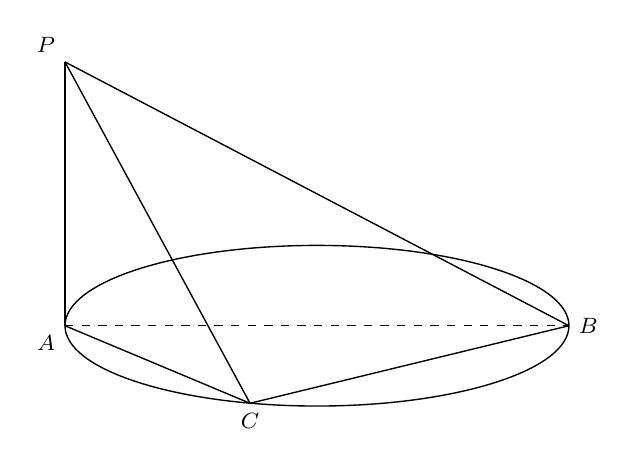
\begin{tikzpicture}[font=\footnotesize, line width=0.5pt, scale=1]
  \coordinate (A) at (-3.2,0);
  \coordinate (B) at (3.2,0);
  \coordinate (C) at (-0.85,-0.985);
  \coordinate (P) at (-3.2,3.35);
  % 底面圆（斜二测画法下的椭圆）
  \draw (0,0) ellipse (3.2 and 1.02);
  % 可见棱
  \draw (P) -- (A);
  \draw (P) -- (B);
  \draw (P) -- (C);
  \draw (A) -- (C);
  \draw (C) -- (B);
  % 被遮挡的直径
  \draw[dashed] (A) -- (B);
  % 点与标签
  \node[above left] at (P) {$P$};
  \node[below left] at (A) {$A$};
  \node[right] at (B) {$B$};
  \node[below] at (C) {$C$};
\end{tikzpicture}
